\section{Experimentation and Results}

\subsection{Similarity Baselines}

Table~\ref{tab:baselines} presents BLEU, ROUGE-L, and BERTScore between $T_0$ and each paraphrased tier. Figure~\ref{fig:decay} visualizes the aggregate decay.

\begin{table}[h]
\centering
\small
\begin{tabular}{llccc}
\toprule
\textbf{Paraphraser} & \textbf{Metric} & \textbf{T1} & \textbf{T2} & \textbf{T3} \\
\midrule
\multirow{3}{*}{ChatGPT} & BLEU & .195 & .172 & .143 \\
 & ROUGE-L & .503 & .464 & .426 \\
 & BERTScore & .923 & .915 & .907 \\
\midrule
\multirow{3}{*}{PaLM2} & BLEU & .470 & .383 & .338 \\
 & ROUGE-L & .698 & .625 & .584 \\
 & BERTScore & .953 & .943 & .938 \\
\midrule
\multirow{3}{*}{Dipper} & BLEU & .168 & .093 & .061 \\
 & ROUGE-L & .377 & .317 & .257 \\
 & BERTScore & .905 & .888 & .877 \\
\midrule
\multirow{3}{*}{Dipper (High)} & BLEU & .010 & .004 & .002 \\
 & ROUGE-L & .130 & .107 & .091 \\
 & BERTScore & .806 & .804 & .803 \\
\midrule
\multirow{3}{*}{Dipper (Low)} & BLEU & .492 & .369 & .304 \\
 & ROUGE-L & .716 & .628 & .565 \\
 & BERTScore & .953 & .940 & .932 \\
\midrule
\multirow{3}{*}{Pegasus (Full)} & BLEU & .415 & .297 & .252 \\
 & ROUGE-L & .673 & .588 & .540 \\
 & BERTScore & .931 & .914 & .906 \\
\midrule
\multirow{3}{*}{Pegasus (Slight)} & BLEU & .841 & .728 & .638 \\
 & ROUGE-L & .919 & .857 & .804 \\
 & BERTScore & .980 & .967 & .956 \\
\bottomrule
\end{tabular}
\caption{Similarity $T_0$ vs.\ $T_n$. BLEU/ROUGE-L lexical; BERTScore semantic. Corpus means.}
\label{tab:baselines}
\end{table}

\begin{figure}[h]
\centering
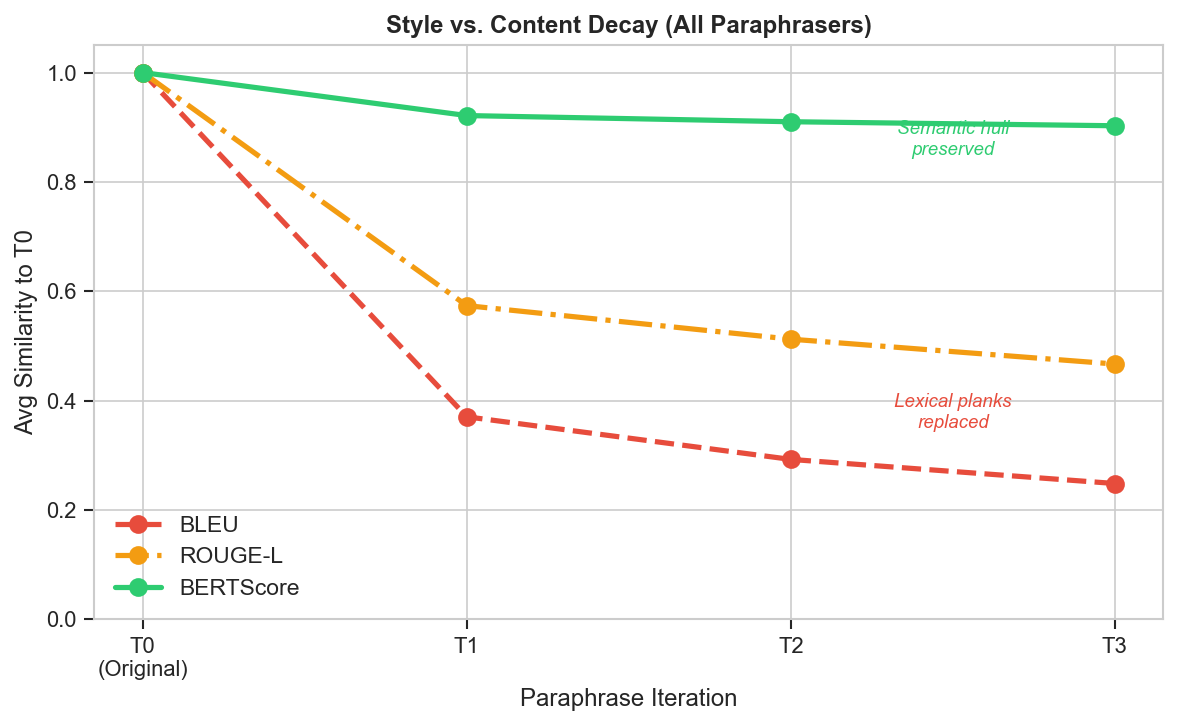
\includegraphics[width=\columnwidth]{figures/baselines/aggregate_style_vs_content.png}
\Description{Line chart showing BERTScore staying above 0.80 while BLEU drops below 0.40 across T0 to T3.}
\caption{Aggregate style vs.\ content decay (RQ1). BERTScore stays above 0.80 while BLEU drops below 0.40 by $T_1$: meaning survives, surface is replaced.}
\label{fig:decay}
\end{figure}

Across all paraphrasers, BERTScore remains 0.80--0.98 while BLEU drops as low as 0.002: meaning is preserved while surface is replaced. The sharpest decay occurs at $T_1$, with only modest additional loss through $T_3$. Within-family variation (Dipper BLEU range: 0.002--0.492) exceeds between-family variation, which is preliminary evidence for RQ3. Exploratory analysis also shows monotonic text compression (279$\rightarrow$184 words) and punctuation erosion across tiers.

\subsection{POS Tag Distributions: Stylistic Drift (RQ1)}

Table~\ref{tab:pos_cosine} reports POS cosine similarity ($T_0$ vs.\ $T_1$) for all seven paraphrasers. The ranking mirrors the lexical ordering from \S5.1.

\begin{table}[h]
\centering
\small
\begin{tabular}{lcc}
\toprule
\textbf{Paraphraser} & \textbf{POS Cosine} & \textbf{Std Dev} \\
\midrule
Pegasus (Slight) & .9922 & .0396 \\
Dipper (Low) & .9840 & .0292 \\
PaLM2 & .9755 & .0385 \\
ChatGPT & .9686 & .0381 \\
Dipper (Default) & .9637 & .0424 \\
Pegasus (Full) & .9626 & .0834 \\
Dipper (High) & .8782 & .0906 \\
\bottomrule
\end{tabular}
\caption{POS cosine ($T_0$ vs.\ $T_1$). Higher = less syntactic restructuring. Even Dipper (High) retains 0.88---grammar is remarkably resilient.}
\label{tab:pos_cosine}
\end{table}

\textbf{Key finding:} Grammatical structure is resilient. Even Dipper (High), which pushes BLEU to 0.002, retains POS cosine 0.878. The spread within the Dipper family alone (0.984--0.878) exceeds the spread across all other model families, reinforcing that \emph{paraphraser configuration matters more than model architecture}.

\subsection{NER Entity Preservation: Content Erasure (RQ1)}

Table~\ref{tab:ner_metrics} presents entity-level metrics for all seven paraphrasers. Articles with zero $T_0$ entities (1,590 of 18,058, or 8.8\%) are excluded from means.

\begin{table}[h]
\centering
\small
\begin{tabular}{lccc}
\toprule
\textbf{Paraphraser} & \textbf{Jaccard} & \textbf{Recall} & \textbf{Precision} \\
\midrule
Pegasus (Slight) & .868 & .887 & .967 \\
PaLM2 & .590 & .658 & .798 \\
Dipper (Low) & .557 & .648 & .734 \\
ChatGPT & .552 & .629 & .766 \\
Pegasus (Full) & .517 & .557 & .846 \\
Dipper (Default) & .330 & .424 & .537 \\
Dipper (High) & .021 & .038 & .059 \\
\bottomrule
\end{tabular}
\caption{NER entity metrics ($T_0$ vs.\ $T_1$). Low Recall = dropping; low Precision = novel-entity introduction. Dipper (High) destroys 96\% of named entities.}
\label{tab:ner_metrics}
\end{table}

\textbf{Key finding:} Entities are far more fragile than grammar. Dipper (High) retains only 3.8\% of original entities (Recall 0.038) while its POS cosine stays at 0.878. This asymmetry answers RQ1: content decays faster than style.

\subsection{Controlled Experiments: The 5.8$\times$ Sensitivity Gap (RQ1)}

Using Dipper Low vs.\ High as a controlled comparison, content features (NER Recall delta: 0.610) are \textbf{5.8$\times$ more sensitive} to paraphrasing intensity than stylistic features (POS cosine delta: 0.104); Figure~\ref{fig:dipper_intensity} visualises the asymmetry. The Pegasus coverage experiment confirms that paraphrasers primarily \emph{shed} entities (Recall $-$0.329) rather than introduce novel ones (Precision $-$0.122).

\begin{figure}[h]
\centering
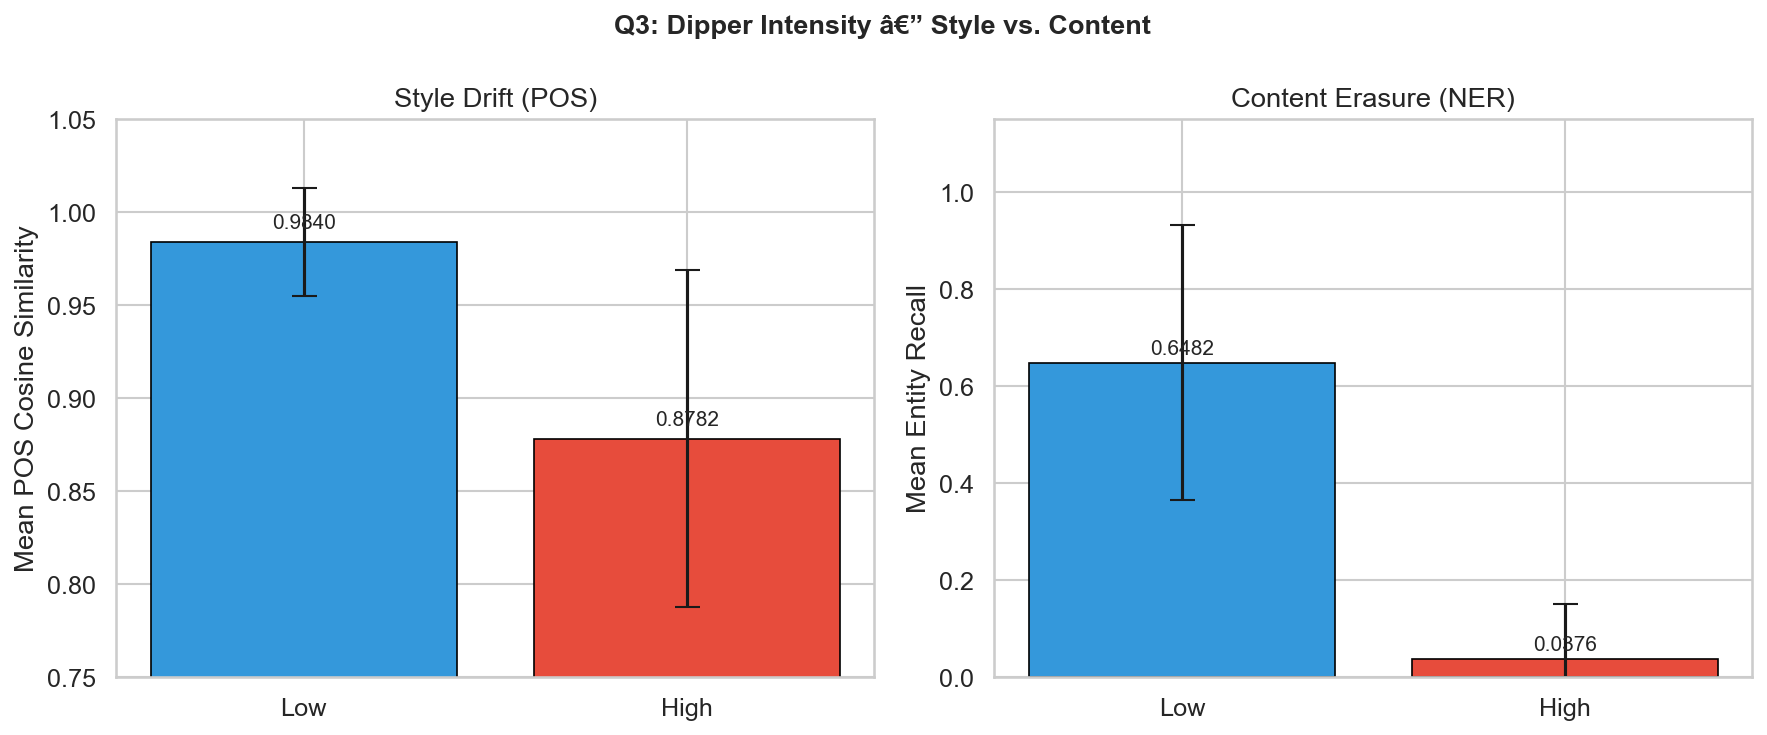
\includegraphics[width=\columnwidth]{figures/fingerprints/q3_dipper_intensity.png}
\Description{Two bar charts comparing Dipper Low vs High: POS cosine drops 0.104, NER Recall drops 0.610.}
\caption{Dipper intensity: content is 5.8$\times$ more sensitive than style (RQ1).}
\label{fig:dipper_intensity}
\end{figure}

\subsection{Paraphraser Fingerprints (RQ3)}

Figure~\ref{fig:fingerprints} plots each paraphraser in style-vs-content space; each occupies a distinct region, confirming identifiable forensic fingerprints.

\begin{figure}[h]
\centering
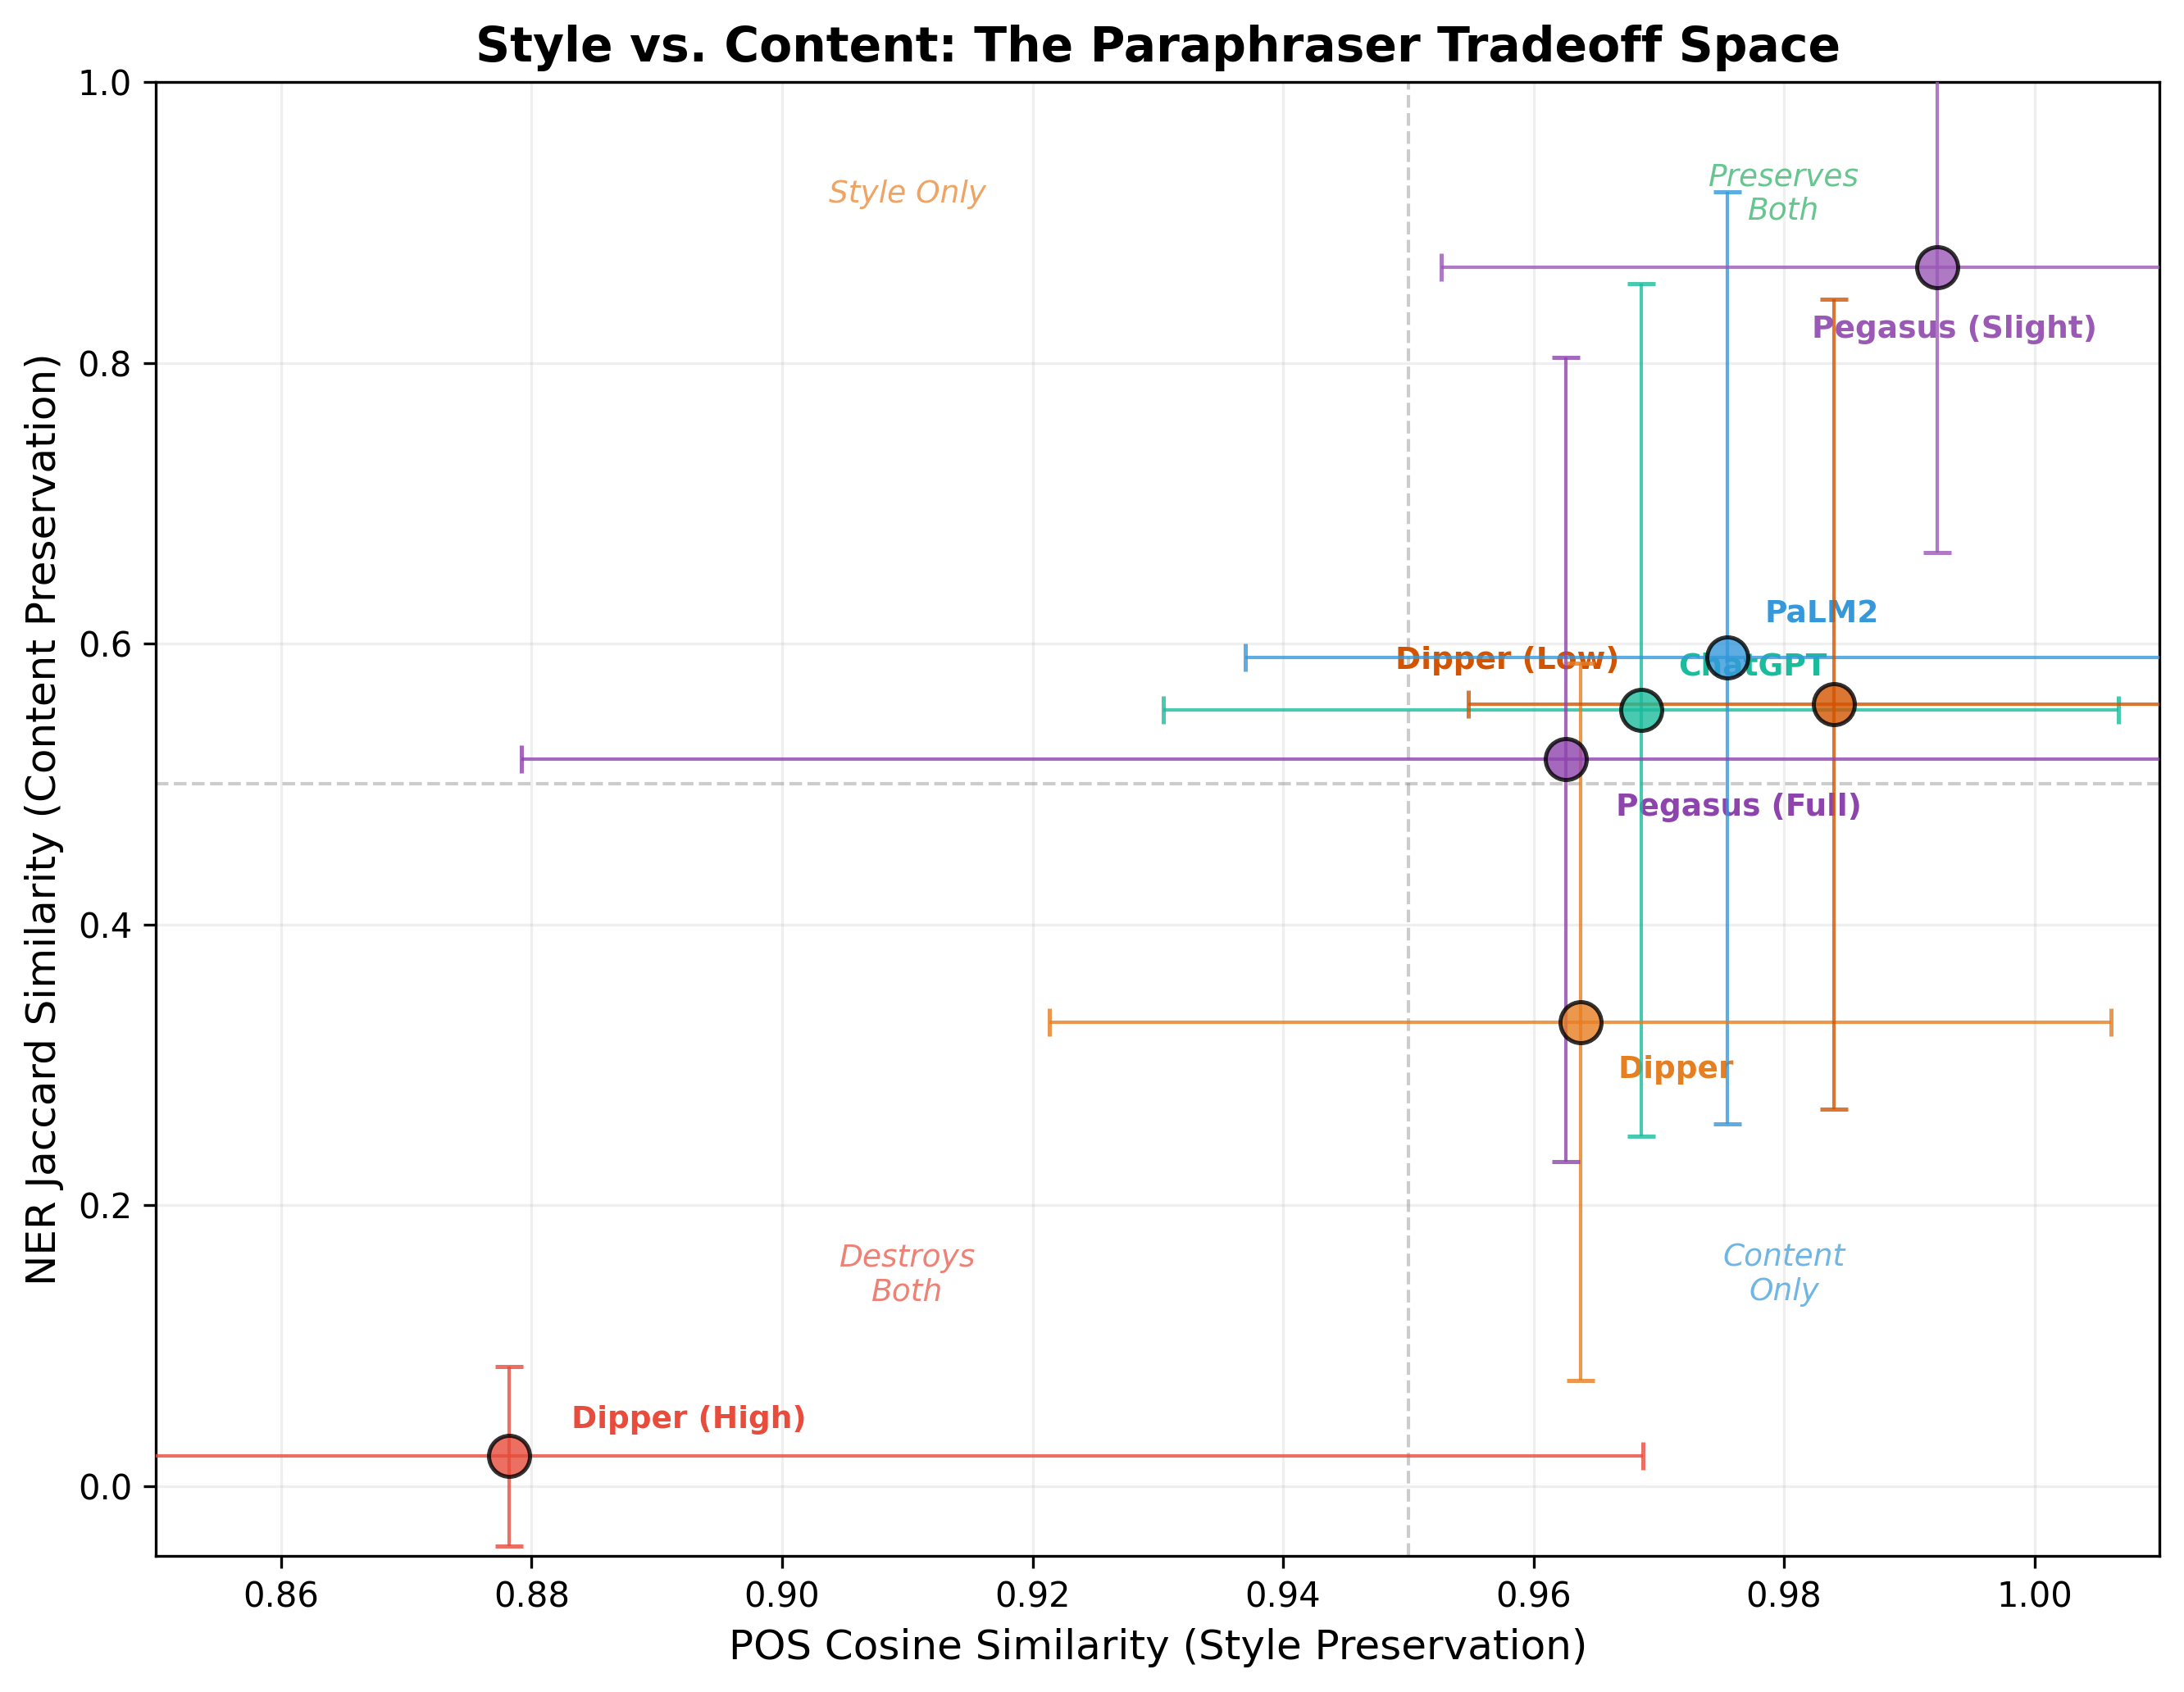
\includegraphics[width=\columnwidth]{figures/fingerprints/style_vs_content_scatter.png}
\Description{Scatter plot showing seven paraphrasers positioned by POS cosine (x-axis) and NER Jaccard (y-axis), with quadrant labels.}
\caption{Paraphrasers in POS cosine (style) vs.\ NER Jaccard (content) space (RQ3). Pegasus (Slight) preserves both; Dipper (High) destroys both; models with similar POS can diverge sharply on NER.}
\label{fig:fingerprints}
\end{figure}

Notably, Pegasus (Full) and Dipper (Default) share POS cosine ($\approx$0.963) but diverge on NER Precision (0.846 vs.\ 0.537): fingerprints are \emph{multi-dimensional}, and combining style and content signals produces separable signatures.

\subsection{Multi-Tier Decay: T0 Through T3 (RQ1)}

Extending to $T_2$ and $T_3$, Table~\ref{tab:multitier} reports POS cosine and NER Recall at every tier; Figure~\ref{fig:composite_decay} visualizes the aggregate pattern.\footnote{T1 values in Tables~\ref{tab:pos_cosine} and \ref{tab:ner_metrics} differ slightly from this table because the multi-tier pivots are aligned per-paraphraser across all four tiers, producing different sample populations (508--3,018 per paraphraser) than the 18,058-row all-paraphrasers pivot.}

\begin{table}[h]
\centering
\small
\begin{tabular}{lcccccc}
\toprule
 & \multicolumn{3}{c}{\textbf{POS Cosine}} & \multicolumn{3}{c}{\textbf{NER Recall}} \\
\cmidrule(lr){2-4} \cmidrule(lr){5-7}
\textbf{Paraphraser} & \textbf{T1} & \textbf{T2} & \textbf{T3} & \textbf{T1} & \textbf{T2} & \textbf{T3} \\
\midrule
Pegasus (Slight) & .993 & .986 & .980 & .892 & .807 & .736 \\
Dipper (Low) & .984 & .979 & .975 & .651 & .567 & .521 \\
PaLM2 & .978 & .974 & .972 & .715 & .672 & .635 \\
ChatGPT & .969 & .966 & .961 & .640 & .606 & .474 \\
Dipper (Default) & .965 & .956 & .948 & .422 & .326 & .272 \\
Pegasus (Full) & .964 & .948 & .938 & .559 & .460 & .418 \\
Dipper (High) & .884 & .863 & .843 & .043 & .018 & .012 \\
\bottomrule
\end{tabular}
\caption{POS cosine and NER Recall ($T_0$ vs.\ $T_n$) across tiers. POS decays gradually; NER Recall drops steeply (Dipper High: 1.2\% at $T_3$).}
\label{tab:multitier}
\end{table}

\begin{figure}[h]
\centering
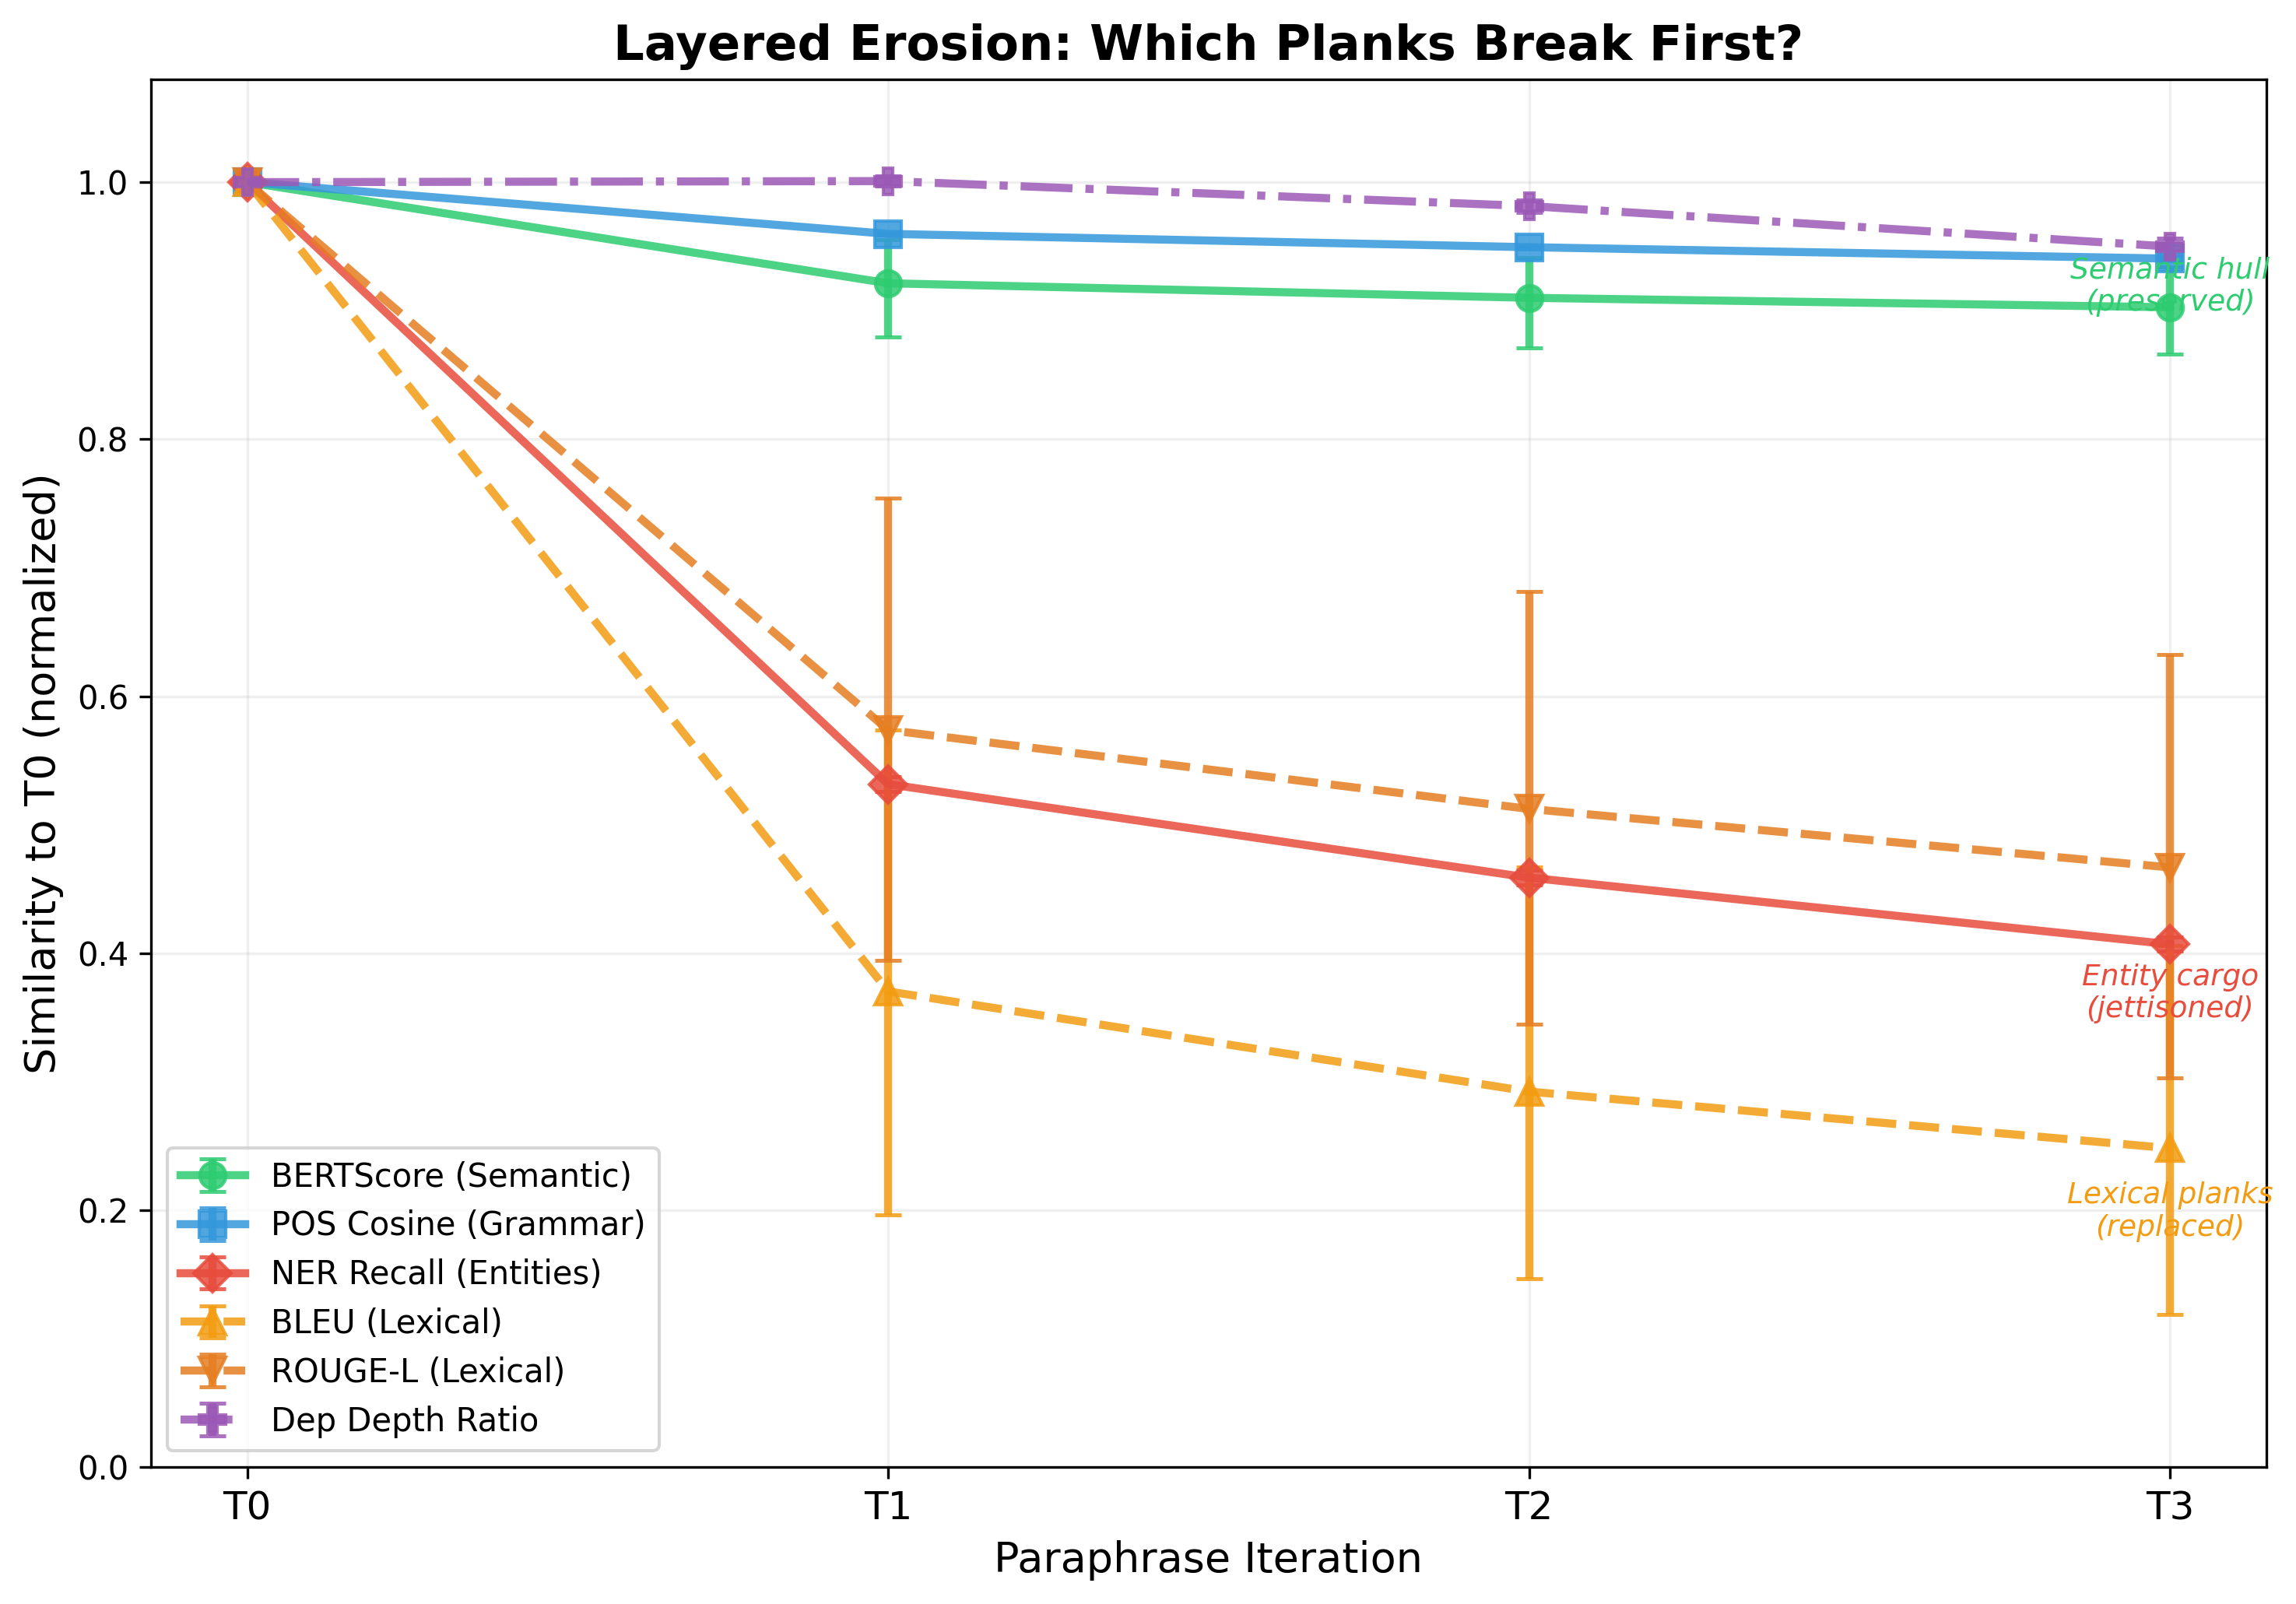
\includegraphics[width=\columnwidth]{figures/baselines/feature_decay_layered.png}
\Description{Line chart showing six features decaying at different rates from T0 to T3: BERTScore and POS cosine stay above 0.90, NER Recall drops to 0.43, BLEU and ROUGE-L collapse below 0.30.}
\caption{Composite feature decay $T_0{\rightarrow}T_3$ aggregated over all paraphrasers (RQ1). Layered erosion: BERTScore and POS cosine stay above 0.90; NER Recall falls to 0.43; BLEU/ROUGE-L collapse below 0.30.}
\label{fig:composite_decay}
\end{figure}

Layered erosion holds at all depths: the ordering BERTScore $>$ POS cosine $>$ NER Recall $>$ ROUGE-L $>$ BLEU is preserved at every tier. Even at $T_3$, Dipper (High) retains POS cosine 0.843 while NER Recall collapses to 1.2\%. Dependency depth is nearly flat across tiers.

\subsection{Authorship Attribution Decay (RQ2)}

Following the protocol in \S4.3, Figure~\ref{fig:attribution_decay} shows F1 decay curves across six paraphrasers and three classifiers. For Logistic Regression, macro F1 drops below the 0.5 random baseline at $T_1$ under Dipper (High): a single aggressive iteration is enough to erase stylometric identity. Pegasus (Slight) retains the most signal, with ensemble methods staying above 0.5 through $T_3$.

\begin{figure}[h]
\centering
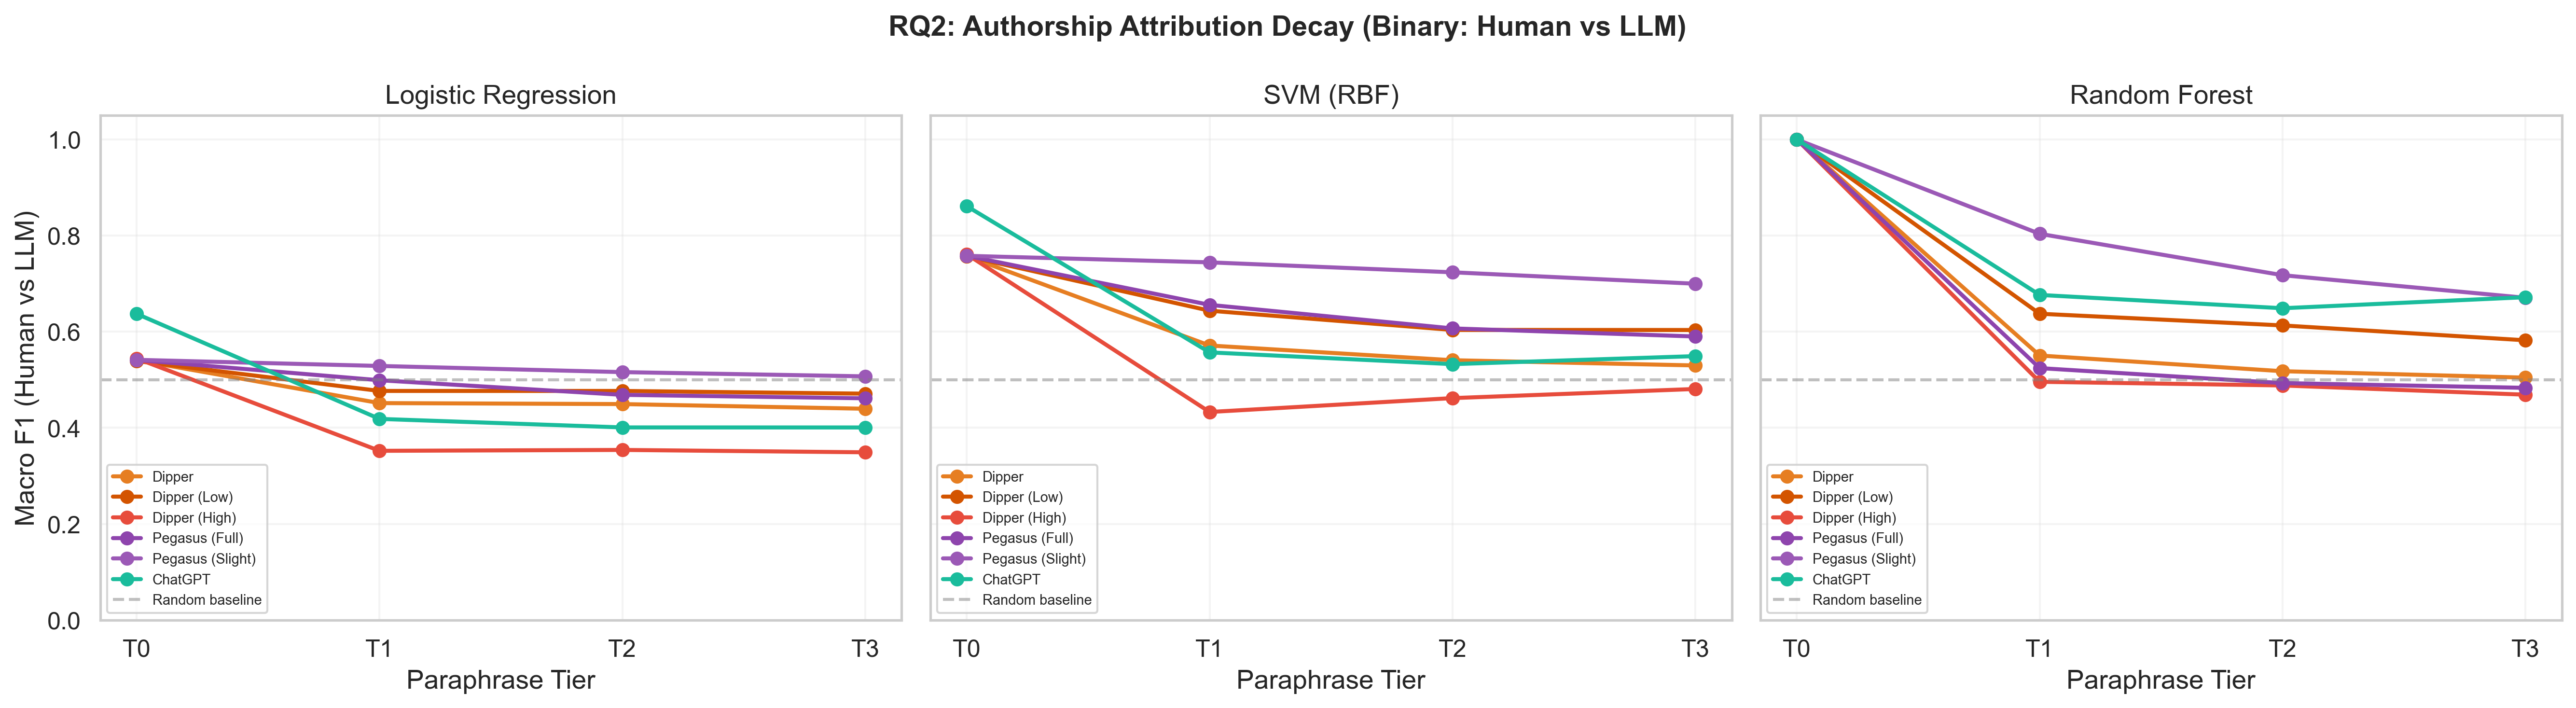
\includegraphics[width=\columnwidth]{figures/fingerprints/attribution_decay_binary.png}
\Description{Three-panel chart showing F1 decay from T0 to T3 for six paraphrasers across Logistic Regression, SVM, and Random Forest classifiers.}
\caption{Binary (Human vs.\ LLM) F1 decay across tiers (RQ2). Dashed gray line is the 0.5 random baseline. Dipper (High) drops below baseline at $T_1$; Pegasus (Slight) retains signal through $T_3$.}
\label{fig:attribution_decay}
\end{figure}

\subsection{Paraphraser Identification (RQ3)}

Following the protocol in \S4.4, SVM (RBF) achieves the highest macro F1 of \textbf{0.755} at 6-class paraphraser identification, confirming that each paraphraser leaves a distinct fingerprint in the delta feature space. Figure~\ref{fig:confusion}: Dipper (High) is most identifiable (93\% correct) while Dipper (Low) is most confusable with Dipper Default.

\begin{figure}[h]
\centering
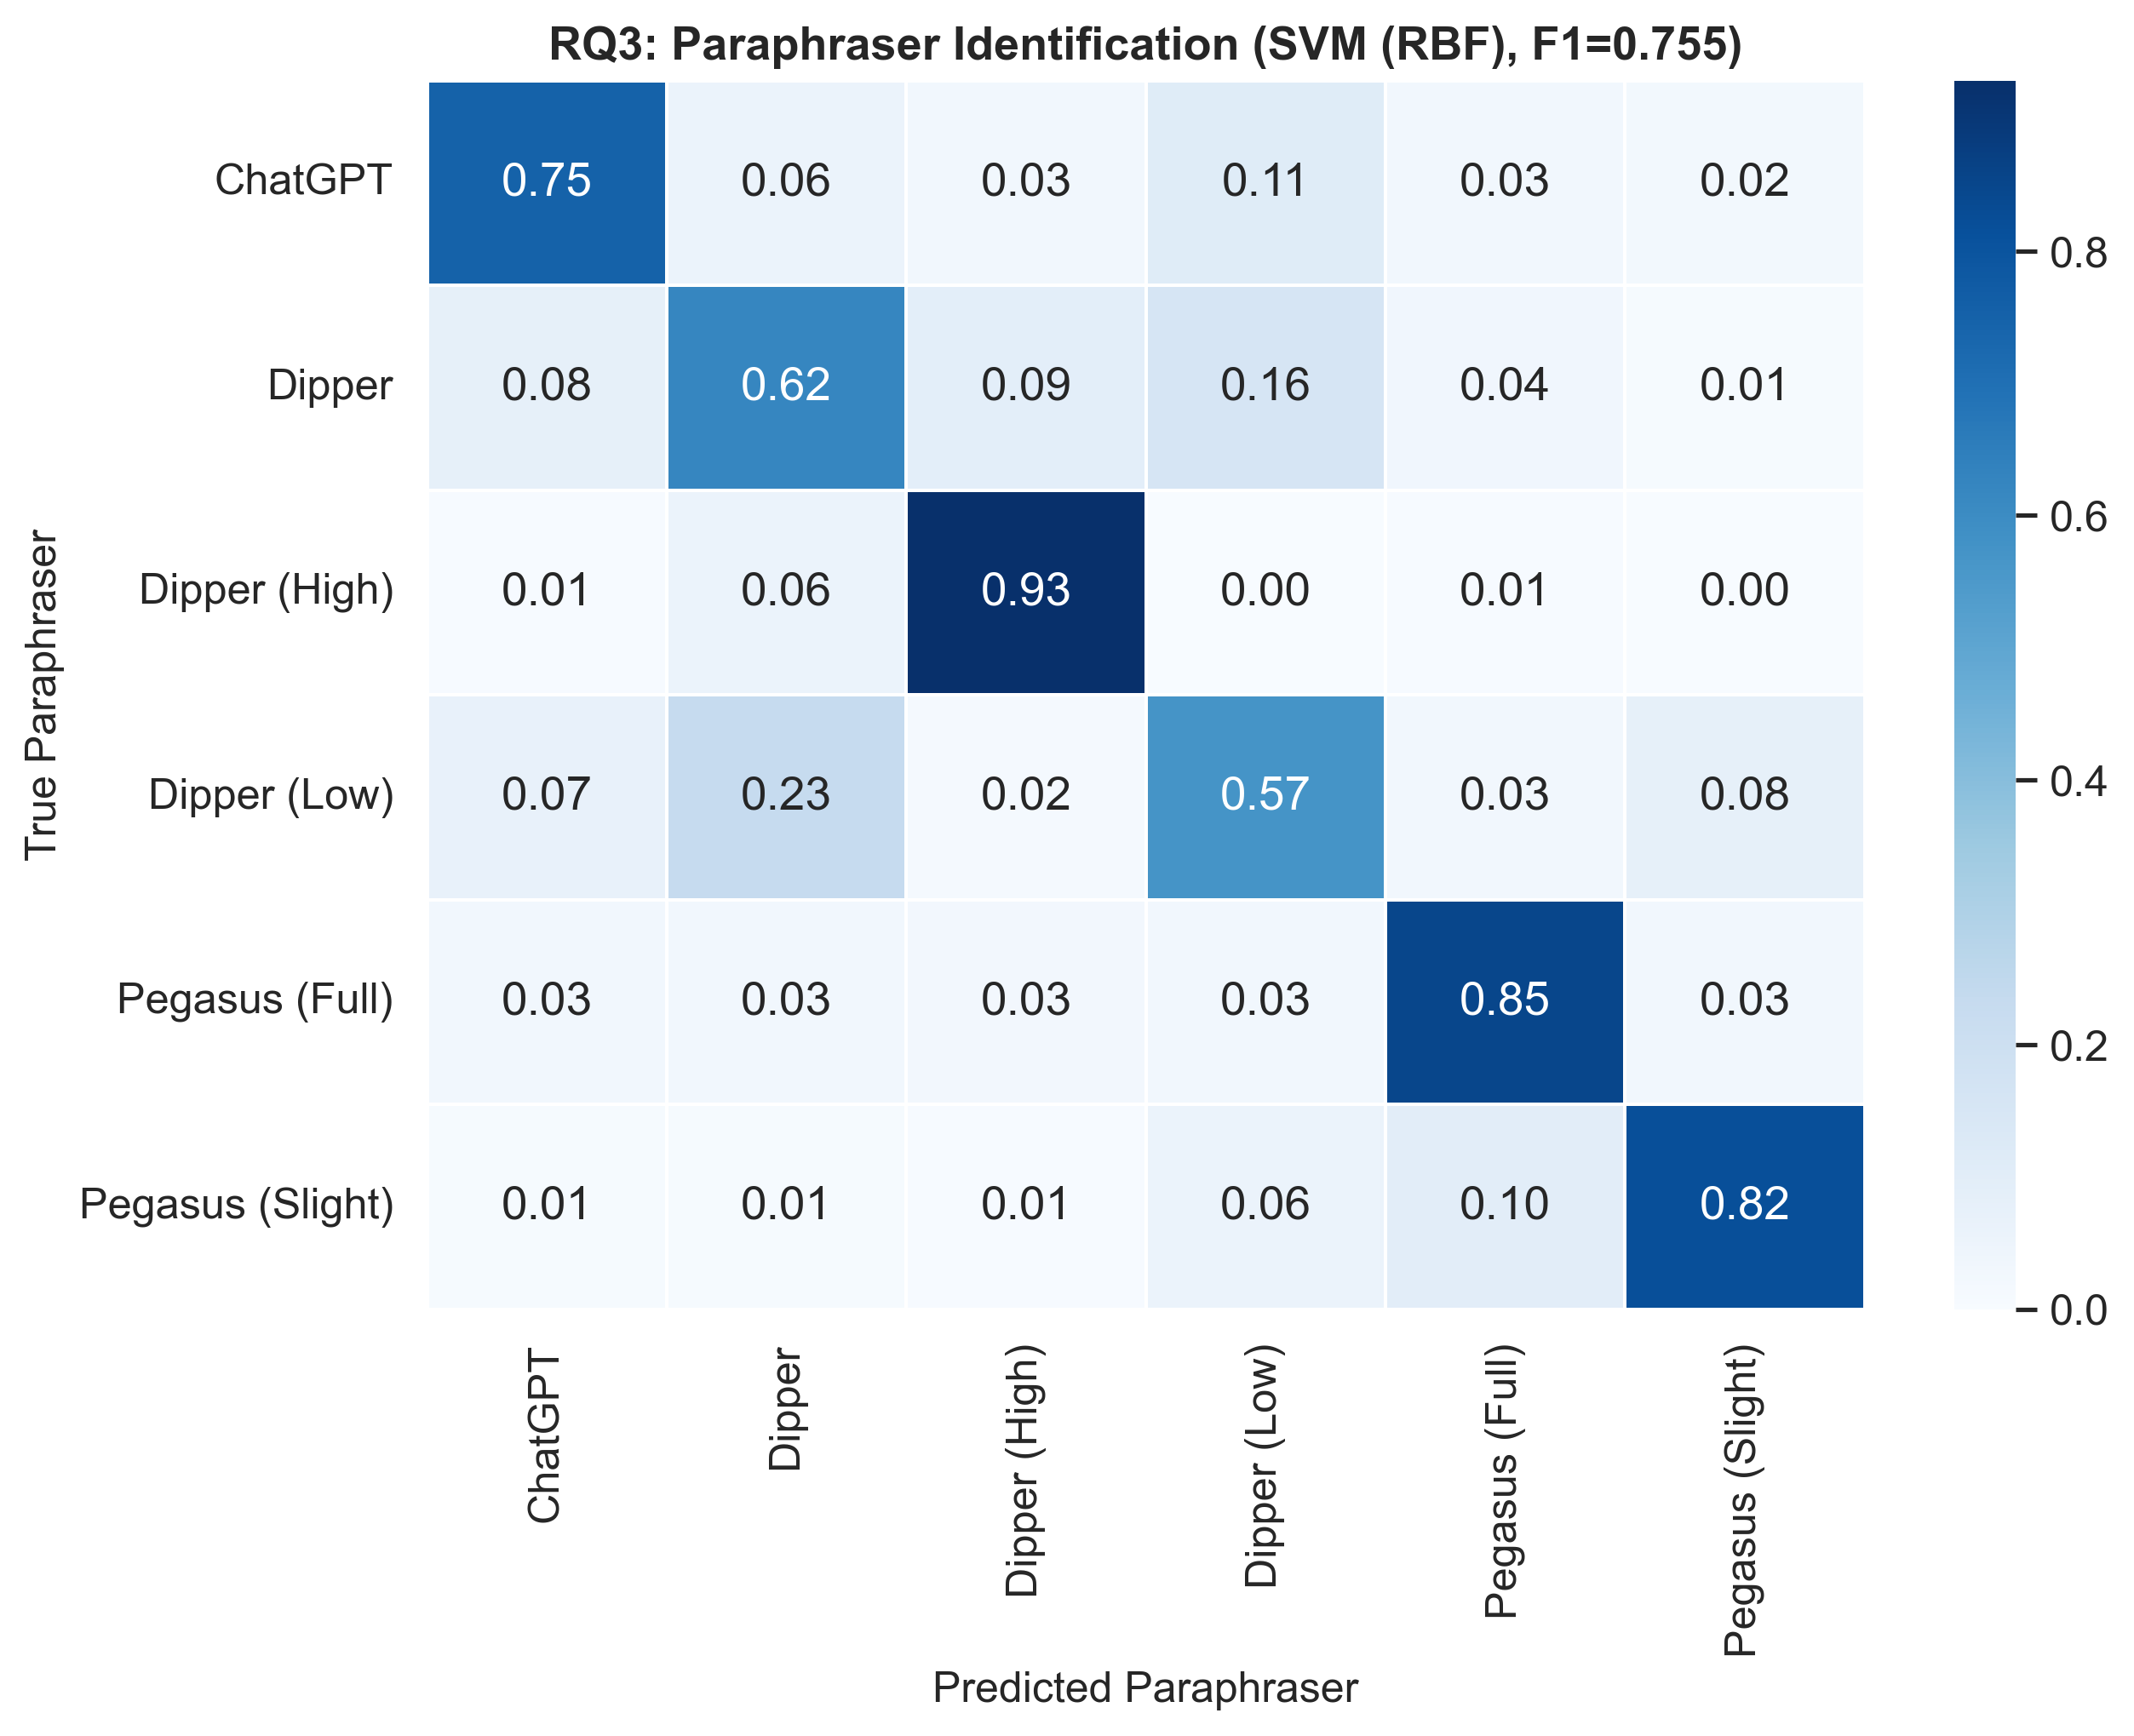
\includegraphics[width=\columnwidth]{figures/fingerprints/paraphraser_confusion_matrix.png}
\Description{Confusion matrix showing 6-class paraphraser identification accuracy. Dipper High is 93 percent correct; Dipper Low is 57 percent correct.}
\caption{6-class paraphraser confusion matrix (SVM, macro F1 = 0.755, RQ3). Dipper (High) most distinctive; Pegasus variants well-separated from Dipper.}
\label{fig:confusion}
\end{figure}

Random Forest feature importance (Figure~\ref{fig:importance}) ranks NER Jaccard, word count ratio, and NER Precision as the top three; POS deltas contribute moderately, with AUX and NOUN shifts most informative.

\begin{figure}[h]
\centering
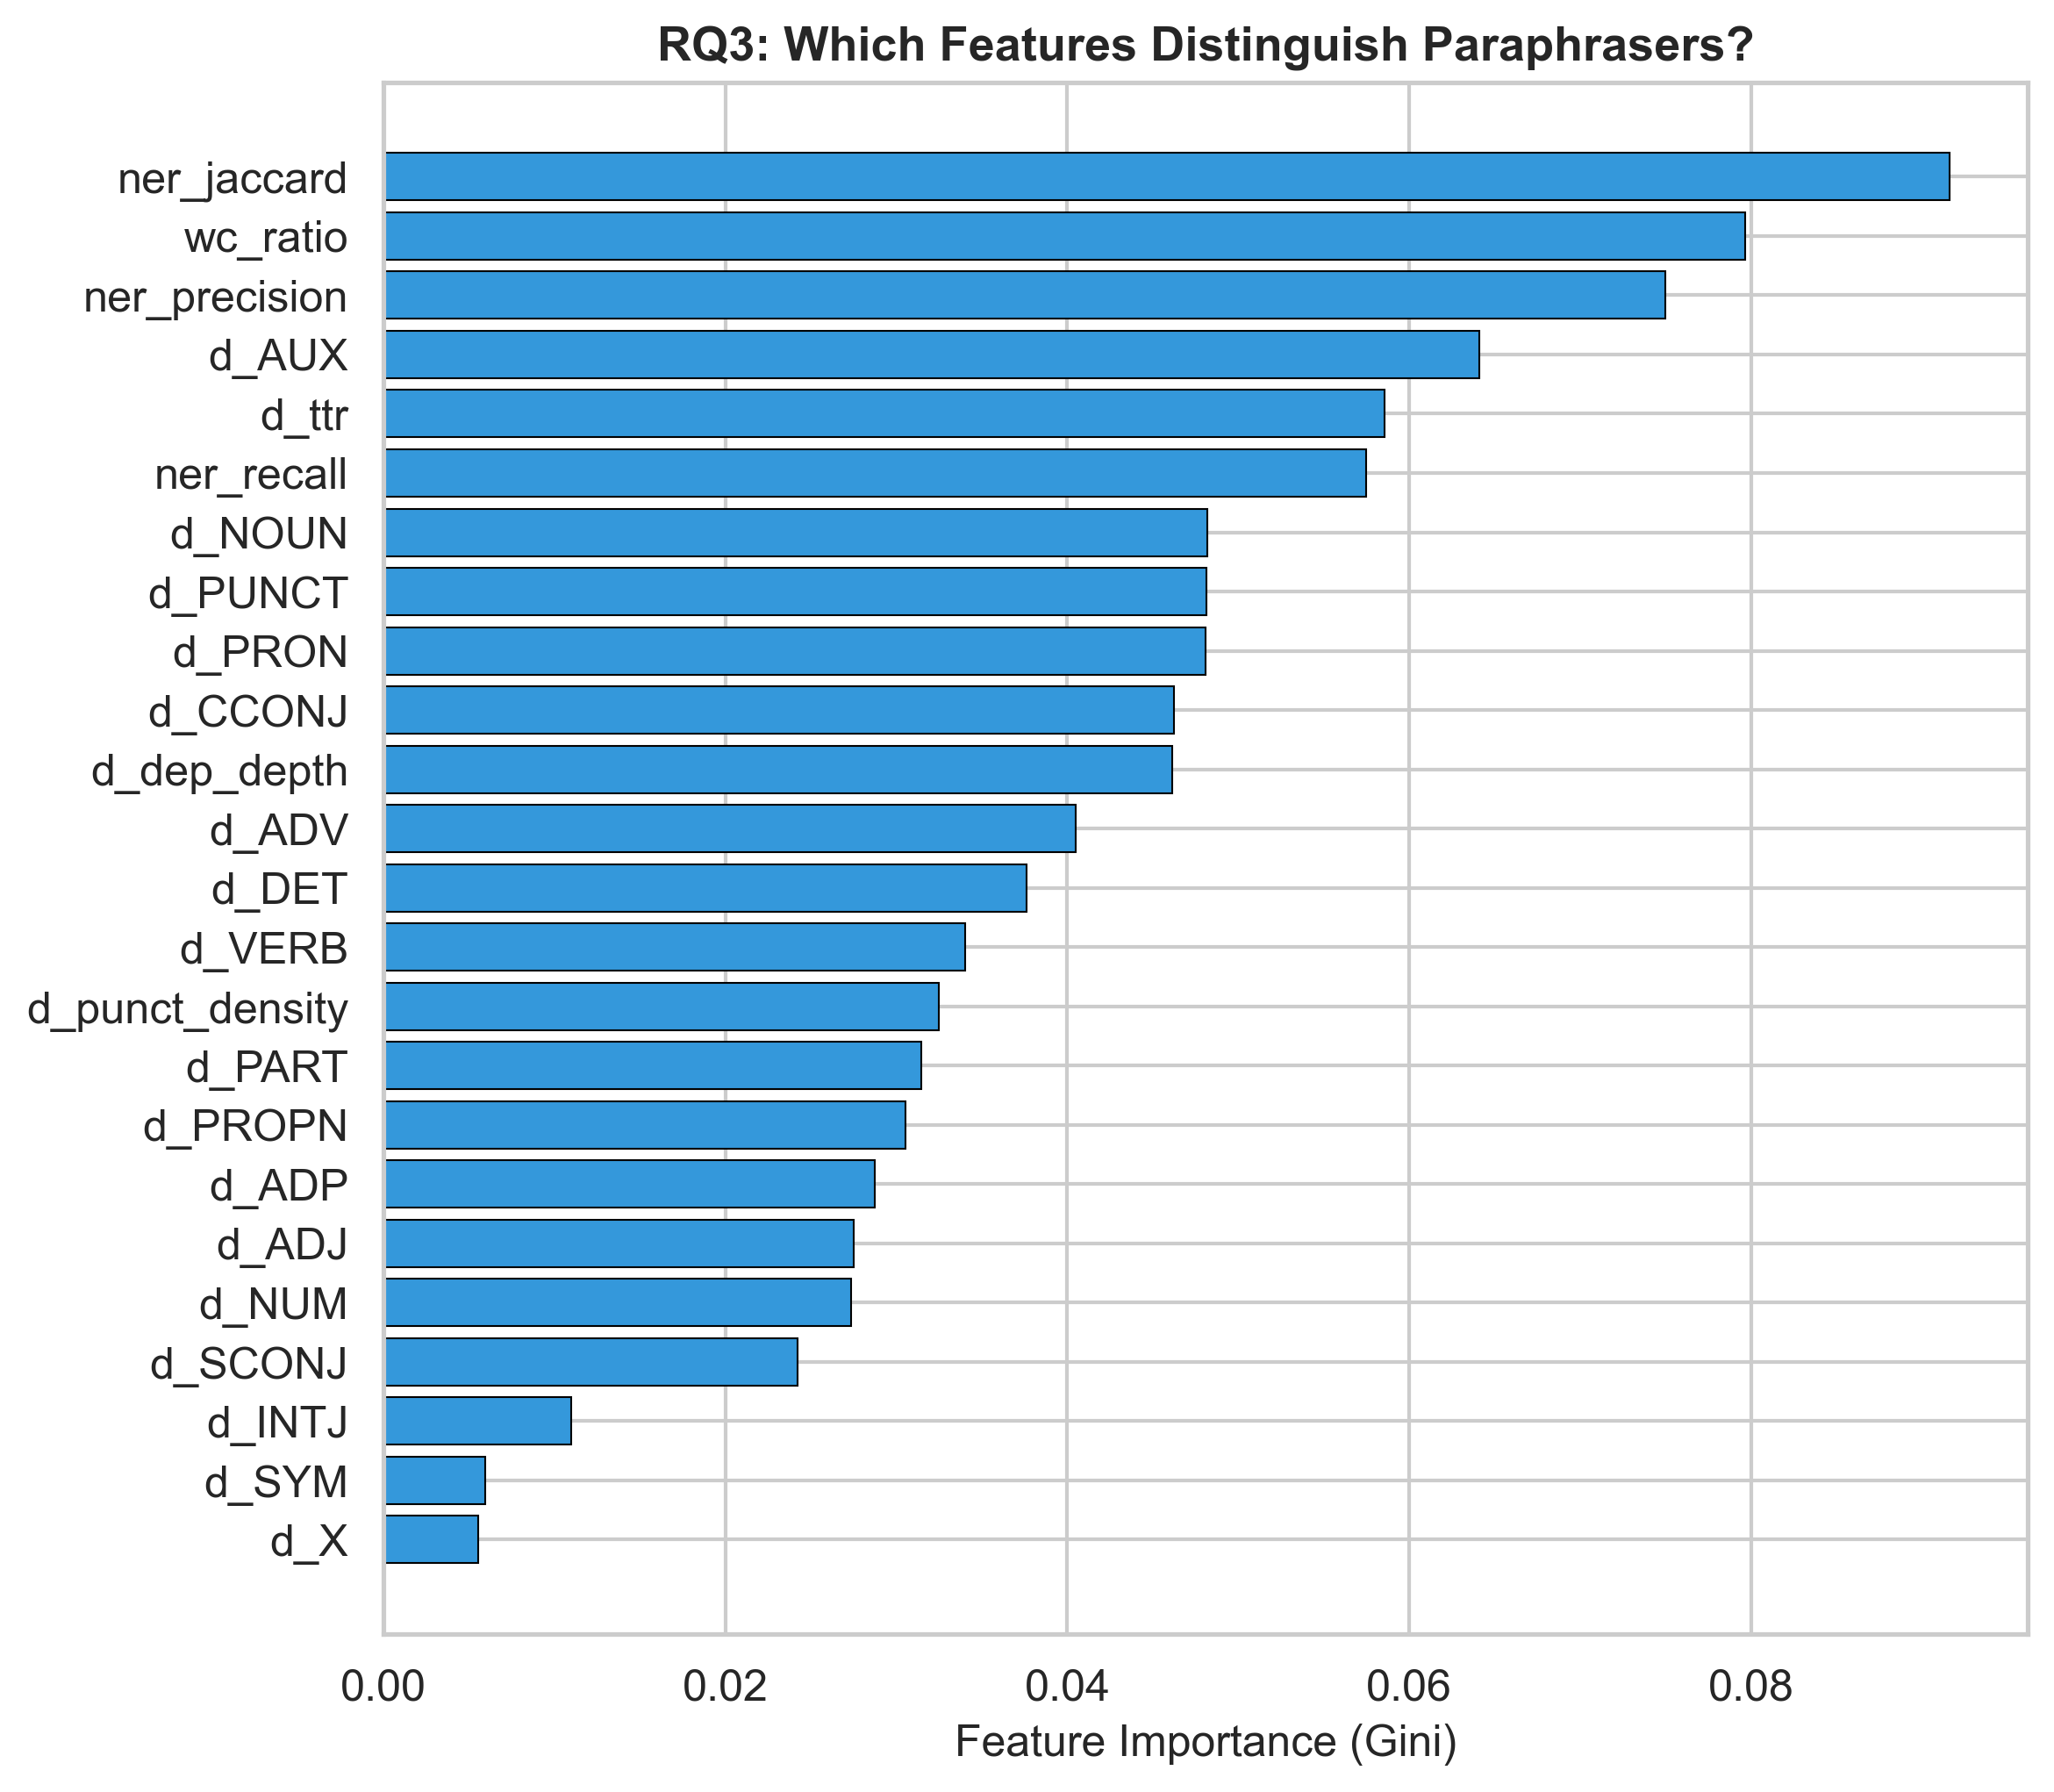
\includegraphics[width=\columnwidth]{figures/fingerprints/paraphraser_feature_importance.png}
\Description{Horizontal bar chart showing feature importance for paraphraser identification. NER Jaccard, word count ratio, and NER Precision are the top three features.}
\caption{Feature importance for paraphraser identification (Random Forest, RQ3). Entity-level features and text compression dominate POS shifts, consistent with the RQ1 finding that content decays faster than style.}
\label{fig:importance}
\end{figure}

\subsection{Domain-Specific Analysis}

Decay varies by domain (Figure~\ref{fig:domain_heatmap}). Entity-rich XSum (18.7 entities/doc) retains NER better (Recall 0.461) than Yelp (5.9 entities, 0.362); CMV has the most resilient POS (0.976); ELI5 attribution collapses nearest chance ($F_1$=0.542 at $T_1$).

\begin{figure}[h]
\centering
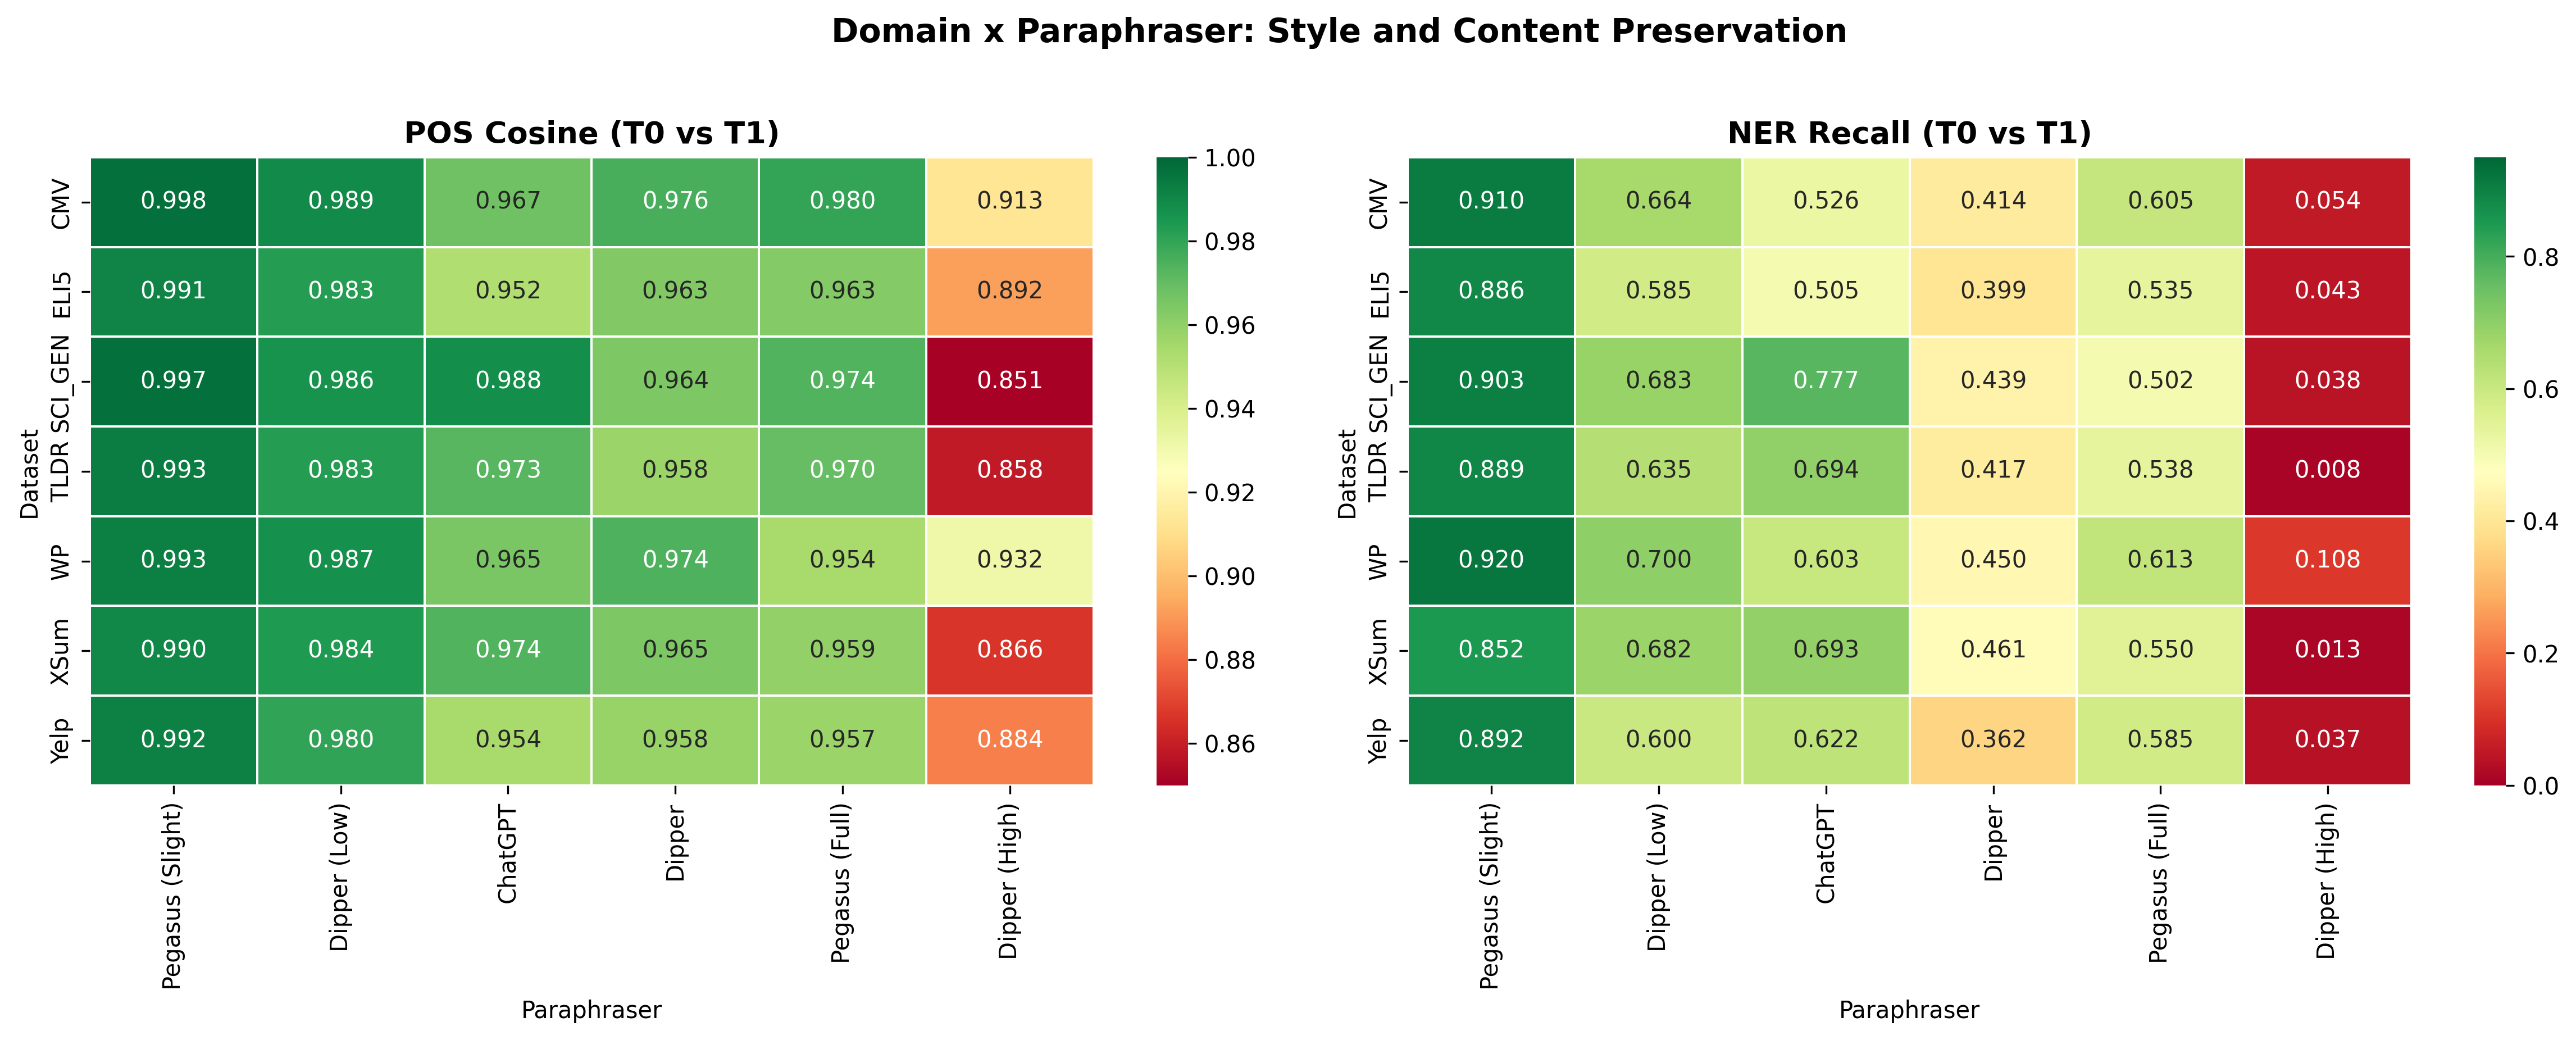
\includegraphics[width=\columnwidth]{figures/domain/domain_paraphraser_heatmap.png}
\Description{Two heatmaps showing POS cosine and NER Recall by dataset and paraphraser.}
\caption{Domain $\times$ paraphraser preservation heatmap (RQ1). Entity-rich domains retain more content; POS resilience is highest in argumentative text.}
\label{fig:domain_heatmap}
\end{figure}

Figure~\ref{fig:domain_attribution} shows domain-wise attribution decay: CMV retains the strongest signal (F1 0.706 at $T_1$), while ELI5 and Yelp collapse toward random by $T_1$. Forensic tools likely need domain-specific calibration.

\begin{figure}[h]
\centering
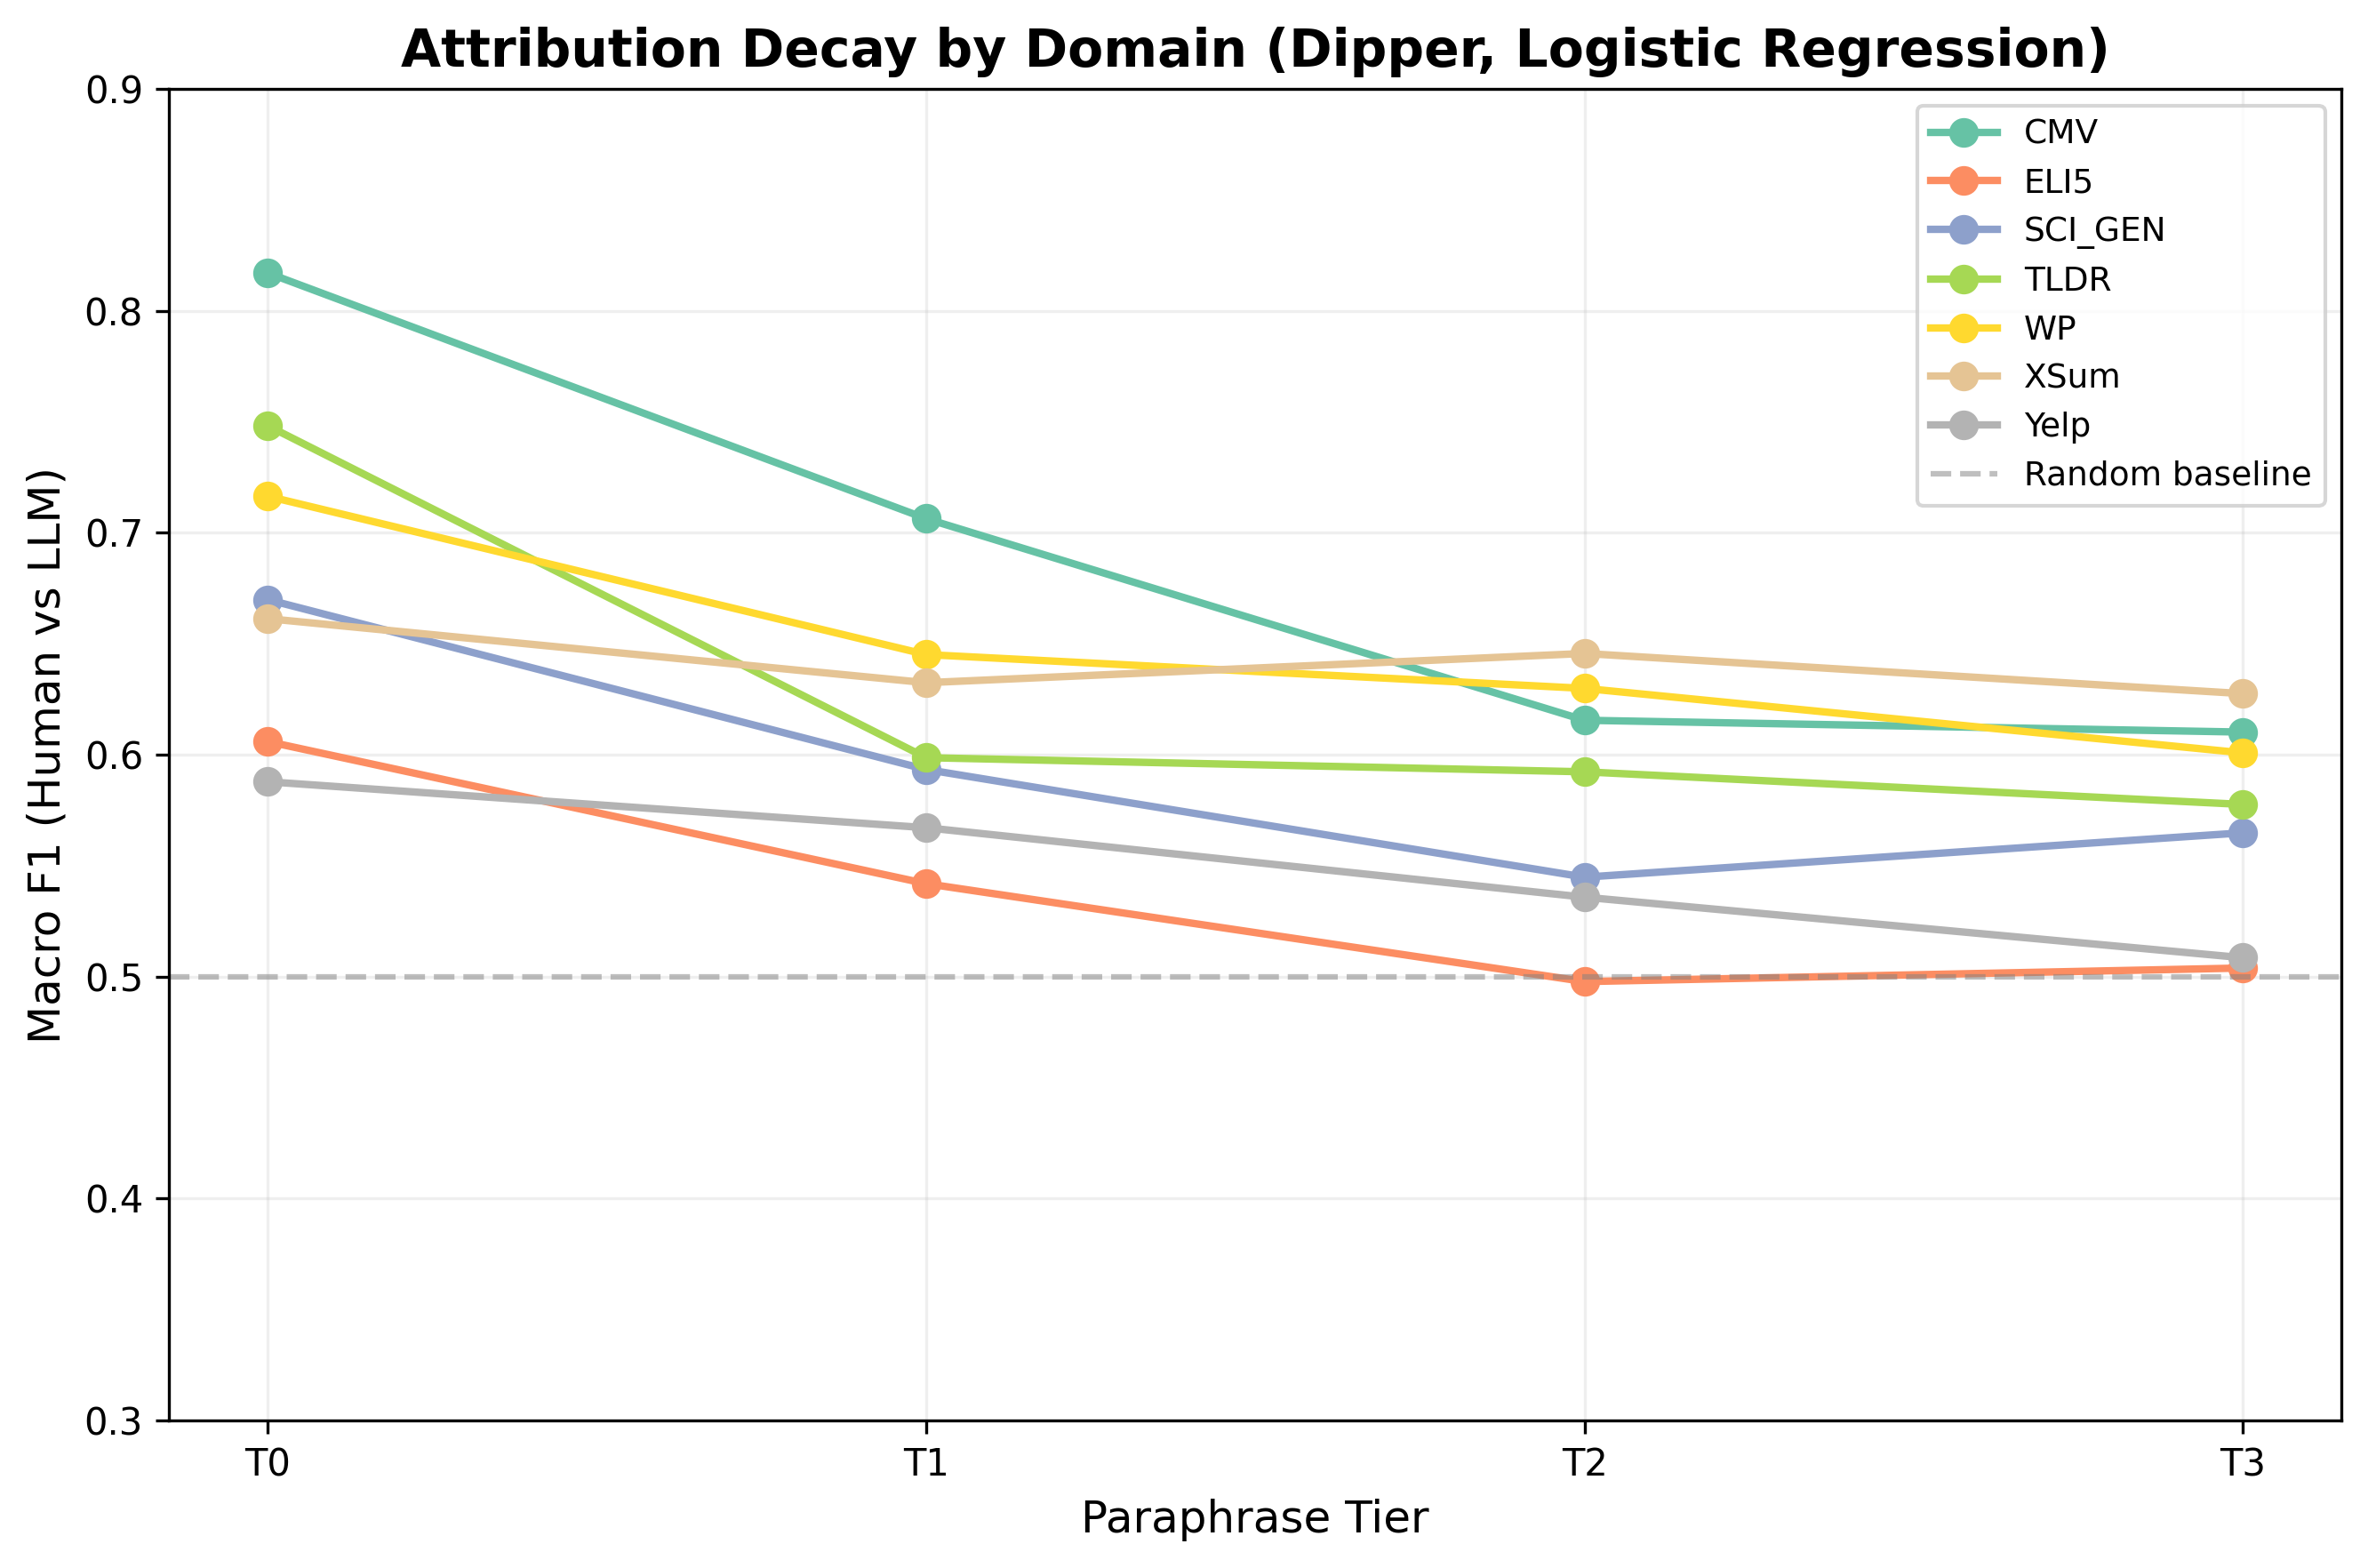
\includegraphics[width=\columnwidth]{figures/domain/domain_attribution_decay.png}
\Description{Line chart showing attribution F1 decay across T0-T3 for seven datasets. CMV and XSum retain the most signal; ELI5 and Yelp collapse toward random.}
\caption{Attribution F1 decay by domain (Dipper, Logistic Regression, RQ2). CMV and XSum retain signal longest; ELI5 and Yelp collapse to random baseline by $T_1$.}
\label{fig:domain_attribution}
\end{figure}

\subsection{Identity Trajectory in Feature Space}

Applying t-SNE to the 23-dim feature vectors at each tier for Dipper (3,010 articles), Figure~\ref{fig:tsne} shows $T_0$ documents occupying a diverse region while $T_3$ clusters into a homogeneous region---visual evidence of convergence toward a machine-normalised style.

\begin{figure}[h]
\centering
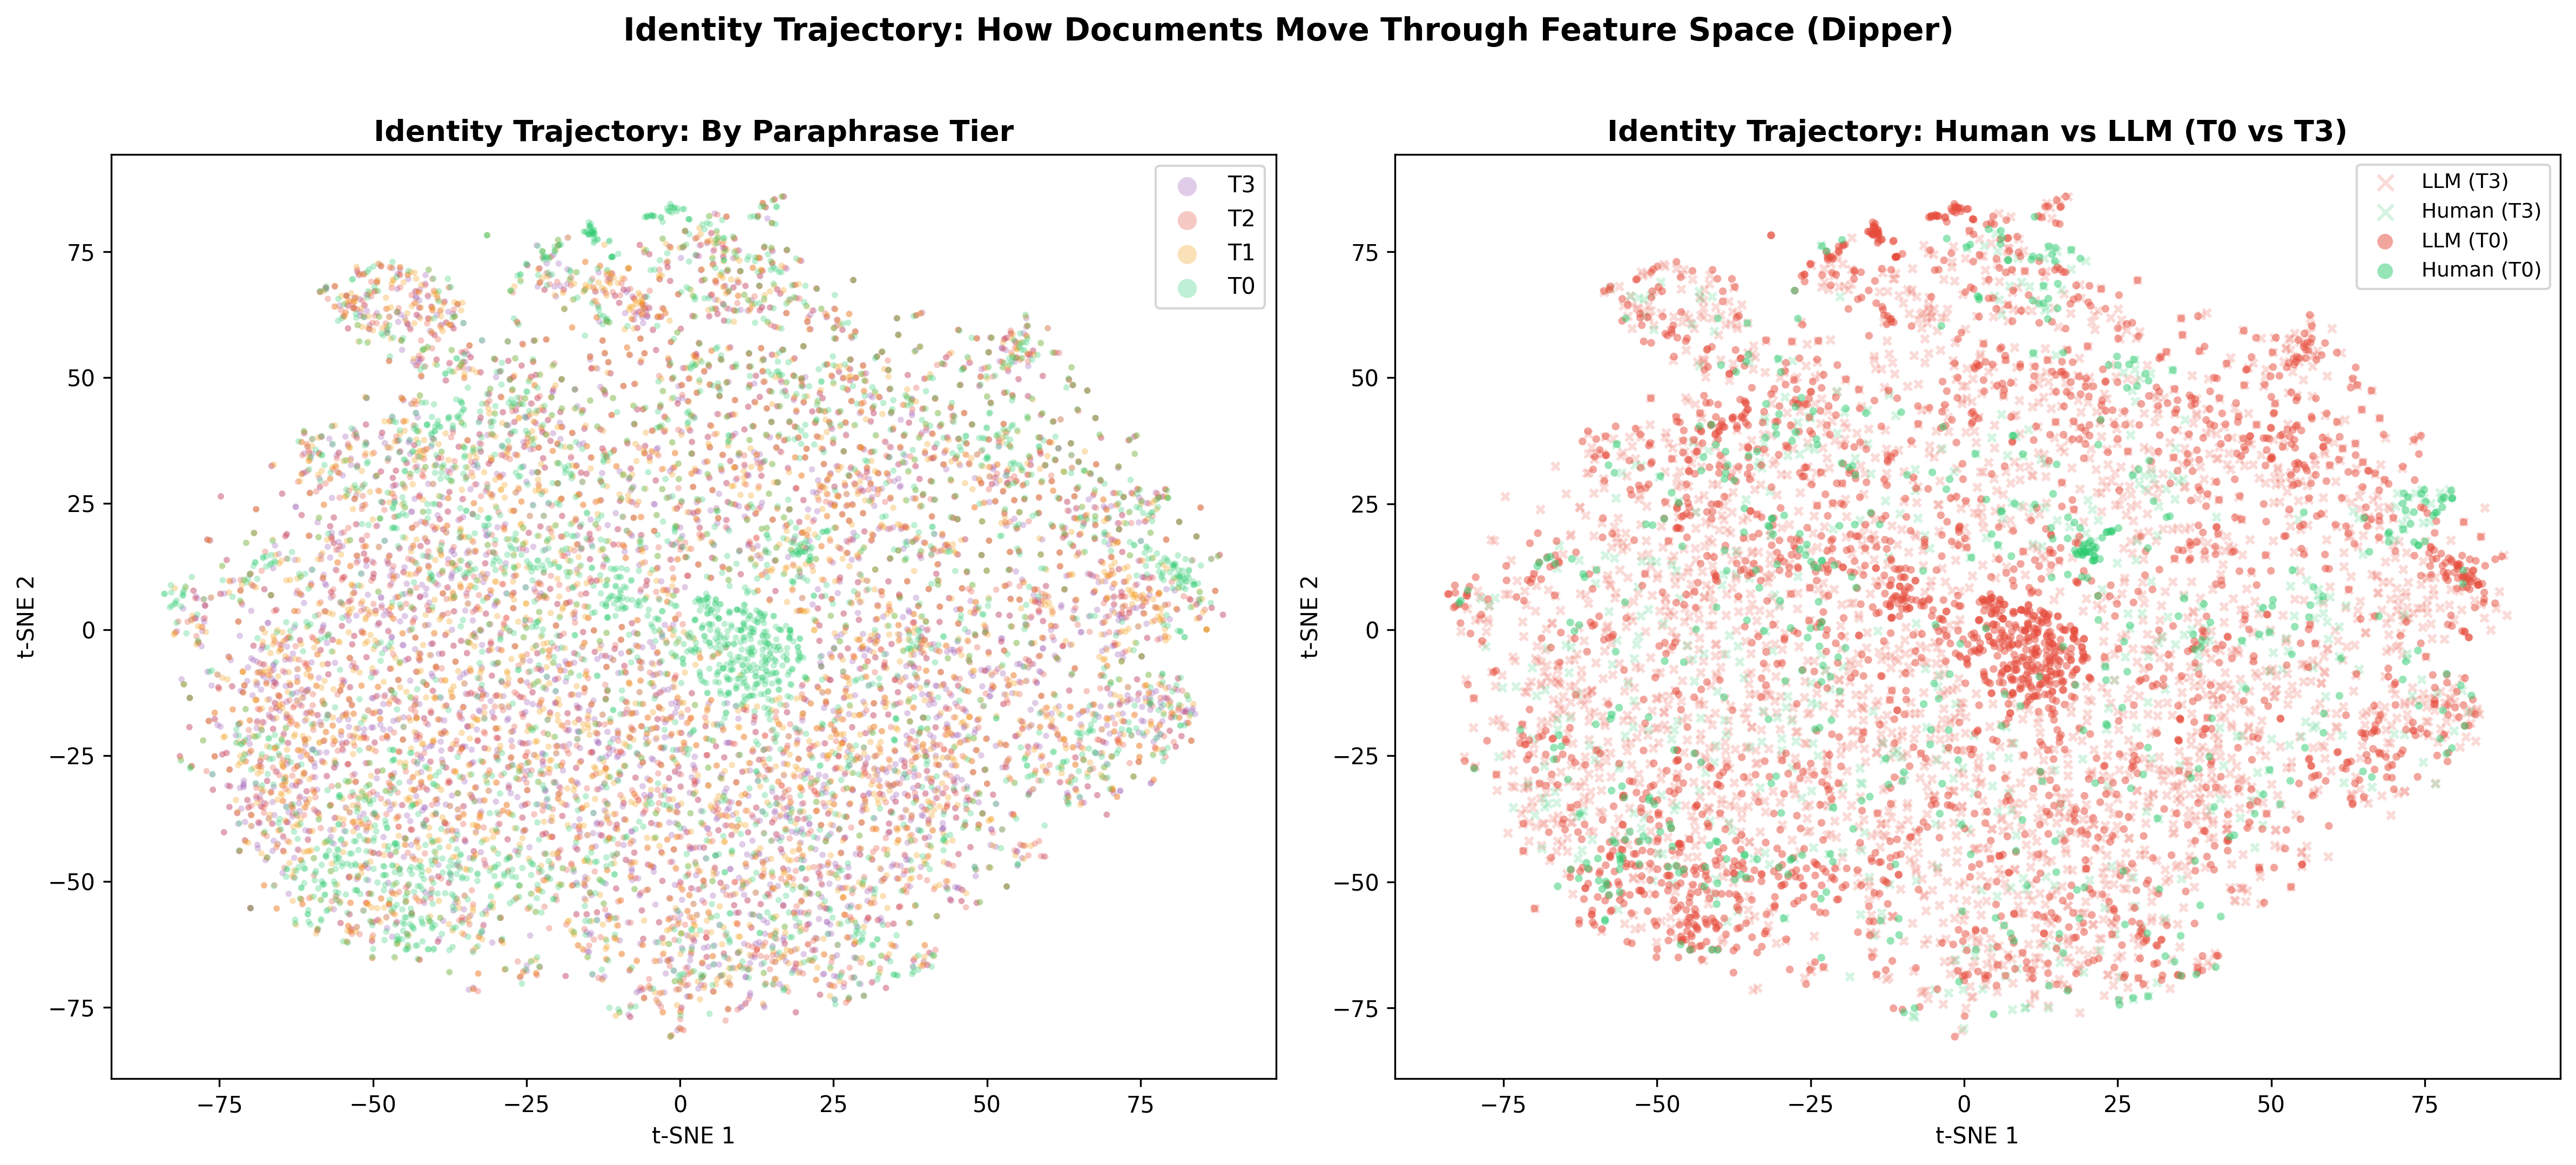
\includegraphics[width=\columnwidth]{figures/fingerprints/identity_trajectory_tsne.png}
\Description{Two t-SNE scatter plots: left colored by paraphrase tier showing T3 clusters more tightly than T0; right showing Human vs LLM centroids converging from T0 to T3.}
\caption{Identity trajectory t-SNE projection (RQ2). Left: colored by tier, showing progressive clustering. Right: Human vs.\ LLM centroids at $T_0$ (circles) and $T_3$ (crosses) converge under paraphrasing.}
\label{fig:tsne}
\end{figure}

To validate the visual impression quantitatively (t-SNE can mislead), we compute silhouette, $k$-NN purity ($k{=}10$), and Human$\leftrightarrow$LLM centroid distance at each tier. All three decline monotonically from $T_0$ to $T_3$ (Figure~\ref{fig:tsne_quant}): centroid distance drops 0.426$\rightarrow$0.287 and $k$-NN purity 0.881$\rightarrow$0.839. Identity is eroding in feature space, not merely compressing visually.

\begin{figure}[h]
\centering
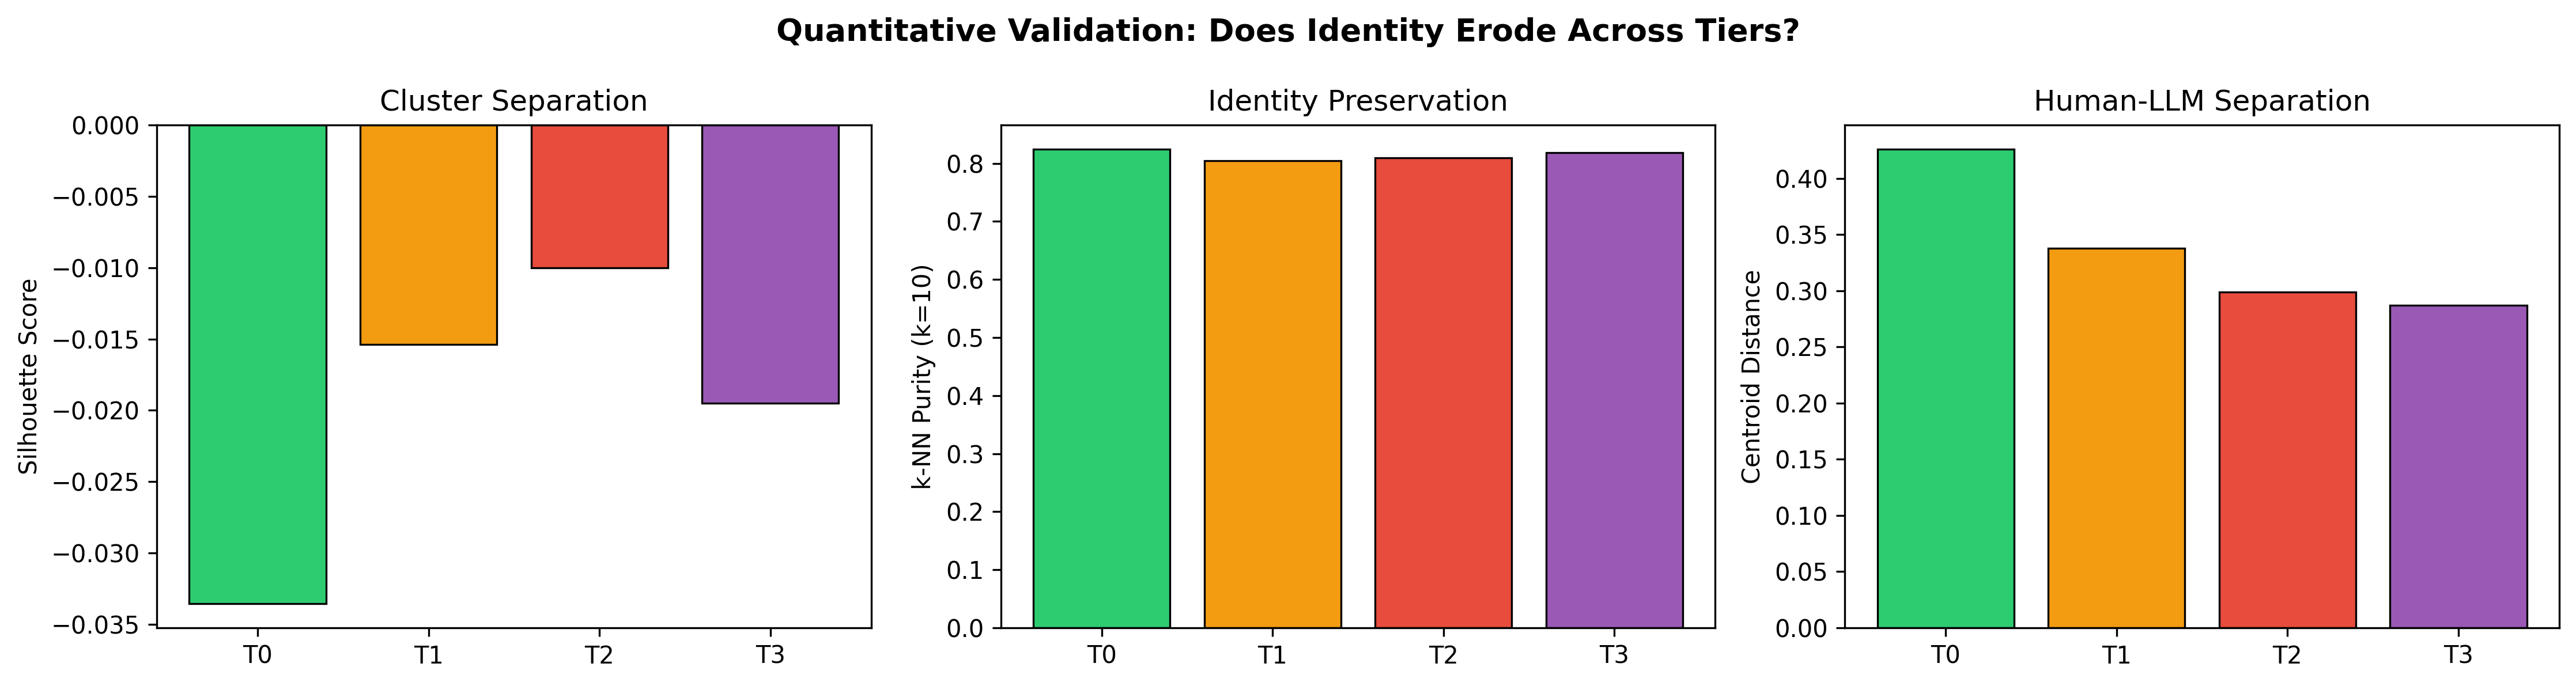
\includegraphics[width=\columnwidth]{figures/fingerprints/identity_quantitative_metrics.png}
\Description{Three bar charts showing silhouette score, k-NN purity, and centroid distance decreasing from T0 to T3.}
\caption{Quantitative validation of identity erosion (RQ2). Silhouette, $k$-NN purity, and Human$\leftrightarrow$LLM centroid distance all decline $T_0{\rightarrow}T_3$.}
\label{fig:tsne_quant}
\end{figure}